\section{Introduction}
\label{sec:introduction}

When evaluating a programming language for use on a project, programmers are faced with an ever-growing array of choices. These choices range from long-lived, well-established languages such as C or Fortran, to the very latest offerings such as Julia or Swift. Selecting a language is a process that is generally rooted in a combination of factors: suitability to the target platform, performance, expressiveness, and (often most importantly) the programmer's familiarity and comfort with the language.

This thesis will be a comparison of the relative strengths of five different programming languages when applied to five different algorithms. To explore this, the problem of large-scale string matching will be examined with a focus on matching DNA-like strings.

\subsection{String Matching}

The topic of string matching has long been a popular area of research in computer science. Before the paper by Knuth, Morris and Pratt in 1977~\cite{knuth} there was already considerable work being done. In the same year, Boyer and Moore~\cite{boyer} published an improvement over the Knuth-Morris-Pratt algorithm with enhancements such as starting the match from the tail of the pattern rather than the head, and allowing for greater right-ward jumps through the string being searched. Even earlier, a 1975 paper by Aho and Corasick~\cite{aho} described a method of searching for multiple patterns simultaneously in a given target string, trading a longer preparation time for the benefit of a construct that could be used over and over on different target strings.

String matching algorithms take many different forms, from simple indexing-based to suffix trees, character comparisons to bit vector operations, and serial to massively-parallel driven by the latest in GPU advances. A search through the Google Scholar service during the preparation of this paper counted nearly 60,000 results matched across diverse disciplines that employ string matching as part of their algorithmic problem-solving processes.

But matching strings means extensive reading and manipulation of strings. These strings are blocks of allocated memory, which can lead to program errors and vulnerabilities. A large percentage of security vulnerabilities discovered in programs are traced back to memory-related issues; in~\cite{cimpanu}, Google software engineers are quoted as attributing roughly 70\% of serious security bugs in Chrome to memory management and safety bugs. The article goes on to report that analysis from Microsoft echoes this number. As such, a process to write programs that are more stable and secure must include careful consideration of memory-related challenges.

\subsection{DNA Strings}

For this study, string matching will be applied to the problem of finding sub-sequences within strings created to emulate DNA (Deoxyribonucleic Acid) sequences. DNA sequence strings have interesting properties, in that they can be \textit{extremely} long but at the same time the alphabet is limited to just four characters (``A'', ``T'', ``C'', and ``G''), called ``bases''.

\begin{figure}[ht]
    \centering
    \begin{minipage}{6in}
        \centering
        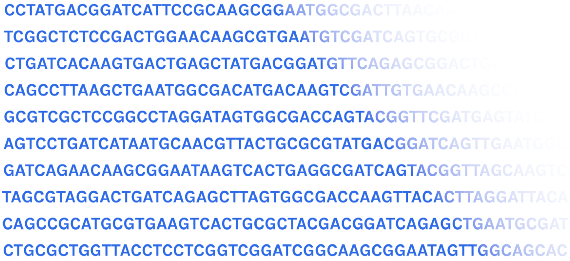
\includegraphics[align=c,height=1in]{figures/dna2.png}
        \hspace*{.2in}
        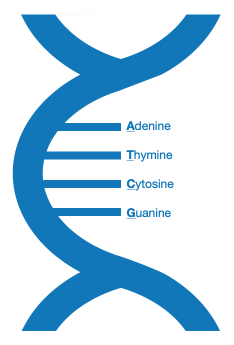
\includegraphics[align=c,height=2in]{figures/dna.png}
    \end{minipage}\hfill
    \caption{DNA and the four bases}
    \label{fig:image:dna}
\end{figure}

In~\cite{heather} Heather and Chain say, ``It is hard to overstate the importance of DNA sequencing to biological research''. Today's researchers use ever-increasing computing resources to process this data faster and in a more complete fashion. String-matching algorithms, mathematical models and other tools have become vital to these research fields, as the size and quantity of data produced by sequencing has also grown. In just the two decades since the completion of the Human Genome Project, current sequencer technology has advanced to the point of being capable of producing as much as a terabyte of data per day~\cite{cabral}.

\subsection{Comparison Bases}
\label{subsec:comparison}

Implementations of the selected algorithms will be developed in five languages: C, C++, Rust, Perl, and Python. Each language's implementations will be evaluated against the others on three bases:

\begin{enumerate}
\item \textbf{Performance}: Run-times for each solution will be gathered using existing timer mechanisms. Time-measurements will be somewhat coarse, as overhead operations such as I/O will necessarily be included in the times.
\item \textbf{Expressiveness}: Each solution will be measured on several source-level metrics in an effort to evaluate the expressiveness of the code.
\item \textbf{Energy efficiency}: Energy usage will be measured for each solution using the Running Average Power Limit (RAPL) tools available on Intel processors. RAPL will be outlined in greater detail in section~\ref{subsubsec:rapl}.
\end{enumerate}

These three bases cover modern concerns in software development: the general performance of an application, the readability/maintainability of the application, and the power consumption of the system running the application. Where the first two criteria are well-known and common, the last has been chosen based on steadily-growing concern over power consumption in the data center industry and in the mobile computing field~\cite{pereira}.
